%% LaTeX-Beamer template for KIT design
%% by Erik Burger, Christian Hammer
%% title picture by Klaus Krogmann
%%
%% version 2.1
%%
%% mostly compatible to KIT corporate design v2.0
%% http://intranet.kit.edu/gestaltungsrichtlinien.php
%%
%% Problems, bugs and comments to
%% burger@kit.edu

\documentclass[18pt]{beamer}
\usepackage[utf8x]{inputenc}
\usepackage{units}
\usepackage{booktabs}

%% CUSTOM
\usepackage{amsmath}
\usepackage{algpseudocode}

%% Definitions
\DeclareMathOperator{\div2}{div}
\renewcommand{\algorithmicrequire}{\textbf{Input:}}
\renewcommand{\algorithmicensure}{\textbf{Output:}}
\algnewcommand\algorithmicto{\textbf{to}}
\algrenewtext{For}[3]{\algorithmicfor\ $#1 \gets #2$ \algorithmicto\ $#3$ \algorithmicdo}
\algnewcommand\algorithmicod{\textbf{od}}
\algrenewtext{EndWhile}{\algorithmicod}
\algrenewtext{EndFor}{\algorithmicod}
%\AtBeginSection[]{%
%\begin{frame}<beamer> % do nothing in handouts
%    \frametitle{Überblick}
%    \tableofcontents[sectionstyle=show/shaded,
%    subsectionstyle=show/show/hide]
%\end{frame}
%}
%\AtBeginSubsection[]{%
%\begin{frame}<beamer> % do nothing in handouts
%    \frametitle{Überblick}
%    \tableofcontents[sectionstyle=show/shaded,
%    subsectionstyle=show/shaded/hide]
%\end{frame}
%}

%% SLIDE FORMAT

% use 'beamerthemekit' for standard 4:3 ratio
% for widescreen slides (16:9), use 'beamerthemekitwide'

\usepackage{templates/beamerthemekit}
%\usepackage{templates/beamerthemekitwide}

 %% TITLE PICTURE

 % if a custom picture is to be used on the title page, copy it into the 'logos'
 % directory, in the line below, replace 'mypicture' with the 
 % filename (without extension) and uncomment the following line
 % (picture proportions: 63 : 20 for standard, 169 : 40 for wide
 % *.eps format if you use latex+dvips+ps2pdf, 
 % *.jpg/*.png/*.pdf if you use pdflatex)


 \titleimage{banner}
 
 
%% Define some colors:
\definecolor{darkblue}{rgb}{0,0,.5}
\definecolor{darkgreen}{rgb}{0,.5,0}

 %% TITLE LOGO

 % for a custom logo on the front page, copy your file into the 'logos'
 % directory, insert the filename in the line below and uncomment it

\titlelogo{logo_150x150}
 
 % (*.eps format if you use latex+dvips+ps2pdf,
 % *.jpg/*.png/*.pdf if you use pdflatex)
 
 %% TikZ INTEGRATION
 
 % use these packages for PCM symbols and UML classes
 % \usepackage{templates/tikzkit}
 % \usepackage{templates/tikzuml}
 
 % the presentation starts here
 
\author{Dominik Muth - dominik.muth@student.kit.edu}
\institute{Institut f\"ur Informatik}


\title[Tutorium 5]{GBI Tutorium Nr. $2^5$}
\subtitle{Tutorium 5}
\date{21. November 2012}

% Bibliography



\begin{document}

	%title page
	\begin{frame}
		\titlepage
	\end{frame}

	%table of contents
	\begin{frame}{Outline/Gliederung}
		\tableofcontents
	\end{frame}
	
	
	\section{\"Ubungsblatt 4}
	\begin{frame} {Übungsblatt 4}
		
	\end{frame}	
		
	
	
	
	\section{Wiederholung} 
	\begin{frame} {Wiederholung - Quiz}
		\begin{itemize}
			\item $A^*$ ist eine formale Sprache! 
			\only<2-> {\color{darkgreen}$\surd$}\\
			\color{black}
			\item $(L_1 \cdot L_2)^* = L_1^* \cdot L_2^*$
			\only<3-> {\color{red}$X$}\\
			\color{black}
			\item $f(x) = x^3-x^2$ ist rechtstotal für $x, f(x) \in \mathbb{R}$.
			\only<4-> {\color{darkgreen}$\surd$}\\
			\color{black}
			\item Eine bijektive Relation ist eine Funktion.
			\only<5-> {\color{darkgreen}$\surd$}\\
			\color{black}
			\item Wenn $f: A \rightarrow B$ injektiv $\Rightarrow f^{-1}$ ist surjektiv.
			\only<6-> {\color{red}$X$}\\
			\color{black}
			\item $A\Rightarrow B \Leftrightarrow \neg B \Rightarrow \neg A$
			\only<7-> {\color{darkgreen}$\surd$}\\
			\color{black}
			\item $(\forall x \exists y \; | \; f(x,y)) \Leftrightarrow (\exists y \forall x \; | \; f(x,y)))$
			\only<8-> {\color{red}$X$}\\
		\end{itemize}
	\end{frame}
	
	
	
	\begin{frame} {Wiederholung - Aufgaben}
		\begin{itemize}
			\item Schreiben sie die Injektivität als prädikatenlogische Formel.
			\pause
			\item Es sei $L \subseteq A^*$ eine formale Sprache. Beweisen oder widerlegen Sie:\\
			$L^+ \cdot L^+ \subseteq L^+$
			\pause
			\item Geben Sie eine formale Sprache $L$ über dem Alphabet $A=\{0,1\}$ an, für welche gilt:\\
				$L$ enthält nur Wörter gerader Parität. 
				Die Parität eines Wortes ist gerade, wenn eine gerade Anzahlen von 1en enthalten sind.
		\end{itemize}
	\end{frame}
	
	
	
	\begin{frame} {Wiederholung}
		\begin{block}{Induktion}
			Alice und Bob feiern ihren Hochzeitstag. Auf ihrer Party befinden sich $n \in \mathbb{N}_+$ Paare.
			Dabei begrüßen sich alle Paare mit Ausnahme des eigenen Partners.\\
			\vspace{10pt}
			a) Geben Sie die Anzahl der Begrüßungen $x_i$ für $i \in \{1,2,3,4,5\}$ Paare an.\\
			\vspace{10pt}
			b) Stellen Sie für $x_n$ eine geschlossene Formel (d.h. einen arithmetischen Ausdruck, in dem nur Zahlen, n und die Grundrechenarten vorkommen) auf.\\
			\vspace{10pt}
			c) Beweisen Sie Ihre Aussage aus Teilaufgabe b) durch vollständige Induktion
		\end{block}
	\end{frame}
	
	
	
	\section{Fragen}
	\begin{frame} {Fragen}
		\begin{itemize}
			\item Fragen zum Stoff?
			\item Fragen zum n\"achsten \"Ubungsblatt?
			\item Generelle Fragen?
			\item Feedback?
		\end{itemize}
	\end{frame}

		
	\begin{frame} {EOF}
		\begin{center}
			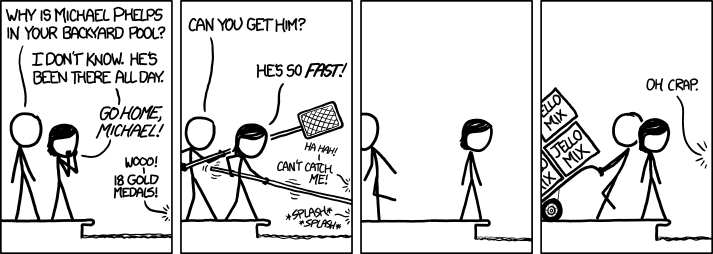
\includegraphics[scale=0.4]{graphics/eof4.png}\\
			\tiny $source: http://imgs.xkcd.com/comics/michael_phelps.png$
		\end{center}
	\end{frame}

\end{document}
